\subsection{Installing an APK} \label{subsection:android-install}
\begin{itemize}
    \item test
\end{itemize}
After having a look at the format of the \gls{apk} and \gls{dex} file format, the application installation is inspected.
Before running an application, it has to be installed.
The installation consists of two steps are applied on the \gls{apk}.
The first step is primarily about verification, while the second step is the bytecode optimization and, in case of \gls{art}, the code compilation.
The differences and procedures of the \gls{dvm} as well as \gls{art} are explained in detail in the following chapters.
Before initiating the installation, the \gls{apk} is checked for a legitimate signature as well as correct classes.dex structure (see figure~\ref{fig:install}).
In case this cannot be verified, the installation is rejected by the OS.
The second step is the optimization where the \gls{odex} version of the classes.dex is generated.
As a reminder, the \gls{odex} is an optimization tailored to the specific architecture of the device in order to achieve the best performance.
This is useful due to the the high diversity of Android running hardware and their different processors.
In the process the classes.dex file is taken from the archive and put as \gls{odex} file into the Dalvik cache.
This is done once and from then on the execution is done by using the \gls{odex} file.
This preprocessed version of the application has an improved startup time. \cite{kovachevaMaster}
The current versions of Android run on the \gls{art}.
For this runtime the second step is more complex since the bytecode has to be compiled an additional time.
This will be explained closer in section~\ref{subsection:android-art}.
\newline
\begin{figure}[h]
    \centering
    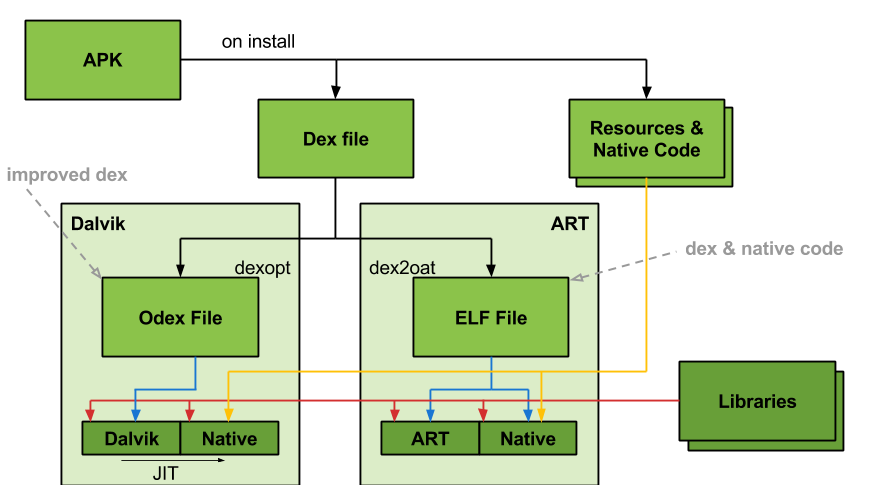
\includegraphics[width=0.8\textwidth]{data/install.png}
    \caption{Installing an \gls{apk} on a device \cite{googleIOArt}}
    \label{fig:install}
\end{figure}

When the application is run later, Android is creating an sandboxed environment for each application.
This is achieved by Android assigning each process a seperate user ID on install to ensure that each application is isolated from the others and has no access on resources except its own. \cite{developerFundamentals}
